\section{Modelling}
\label{sec:modelling}
We took \code{DiffMedianHourlyPercent} and \code{DiffMeanHourlyPercent}  as modelling targets from UK data \cite{gov-uk-gpg-data}, and built models to
predict the pay gap based on a company's features and quartile distributions using supervised regression.  

\paragraph{Modelling methodology}
Because the GPG is generally improving year on year,
we want the year to also be a predictive feature, so we combined training data from all three years. But this means that a company's data from different years may end up split between training and test sets. It will  be similar enough to cause overfitting. To prevent this, we initially withhold 10\% of all companies' data (randomly shuffled and sampled) as a holdout cross-validation set, and only use the remaining 90\% of data during training. We perform 3-fold validation during training and take the average of the scores. After the best models are selected from the test data, we evaluate them using the holdout cross-validation set. 

\paragraph*{Hypothesis} From data exploration and through GPG reports we see the difference in number of women and men in upper quartile and lower quartile to be a potential factor in GPG.

\paragraph*{Feature engineering} The quartile-related data in the raw dataset represents the percentage of each quartile that were men or women. From this, we can derive the relative proportion of men and women in the whole company.
Further, we were able to extract the percentage of men and women in each quartile as a factor of the percentage of men and women in the company, \code{PercMaleWorkforceIn\_X\_Quartile} and \code{PercFemaleWorkforceIn\_X\_Quartile}. For example, if 30\% of employees are female and there are 30\% women in the top quartile, then the representation is not skewed and this should be present in the input data.
\code{RepresentationIn\_X\_QuartileSkew} tells the adjusted representation difference of the employees in a company (Appendix \ref{app:data-dic}, Table \ref{tab:additional-fields}).

\paragraph*{Manifold learning and dimension reduction} 

\begin{centering}
    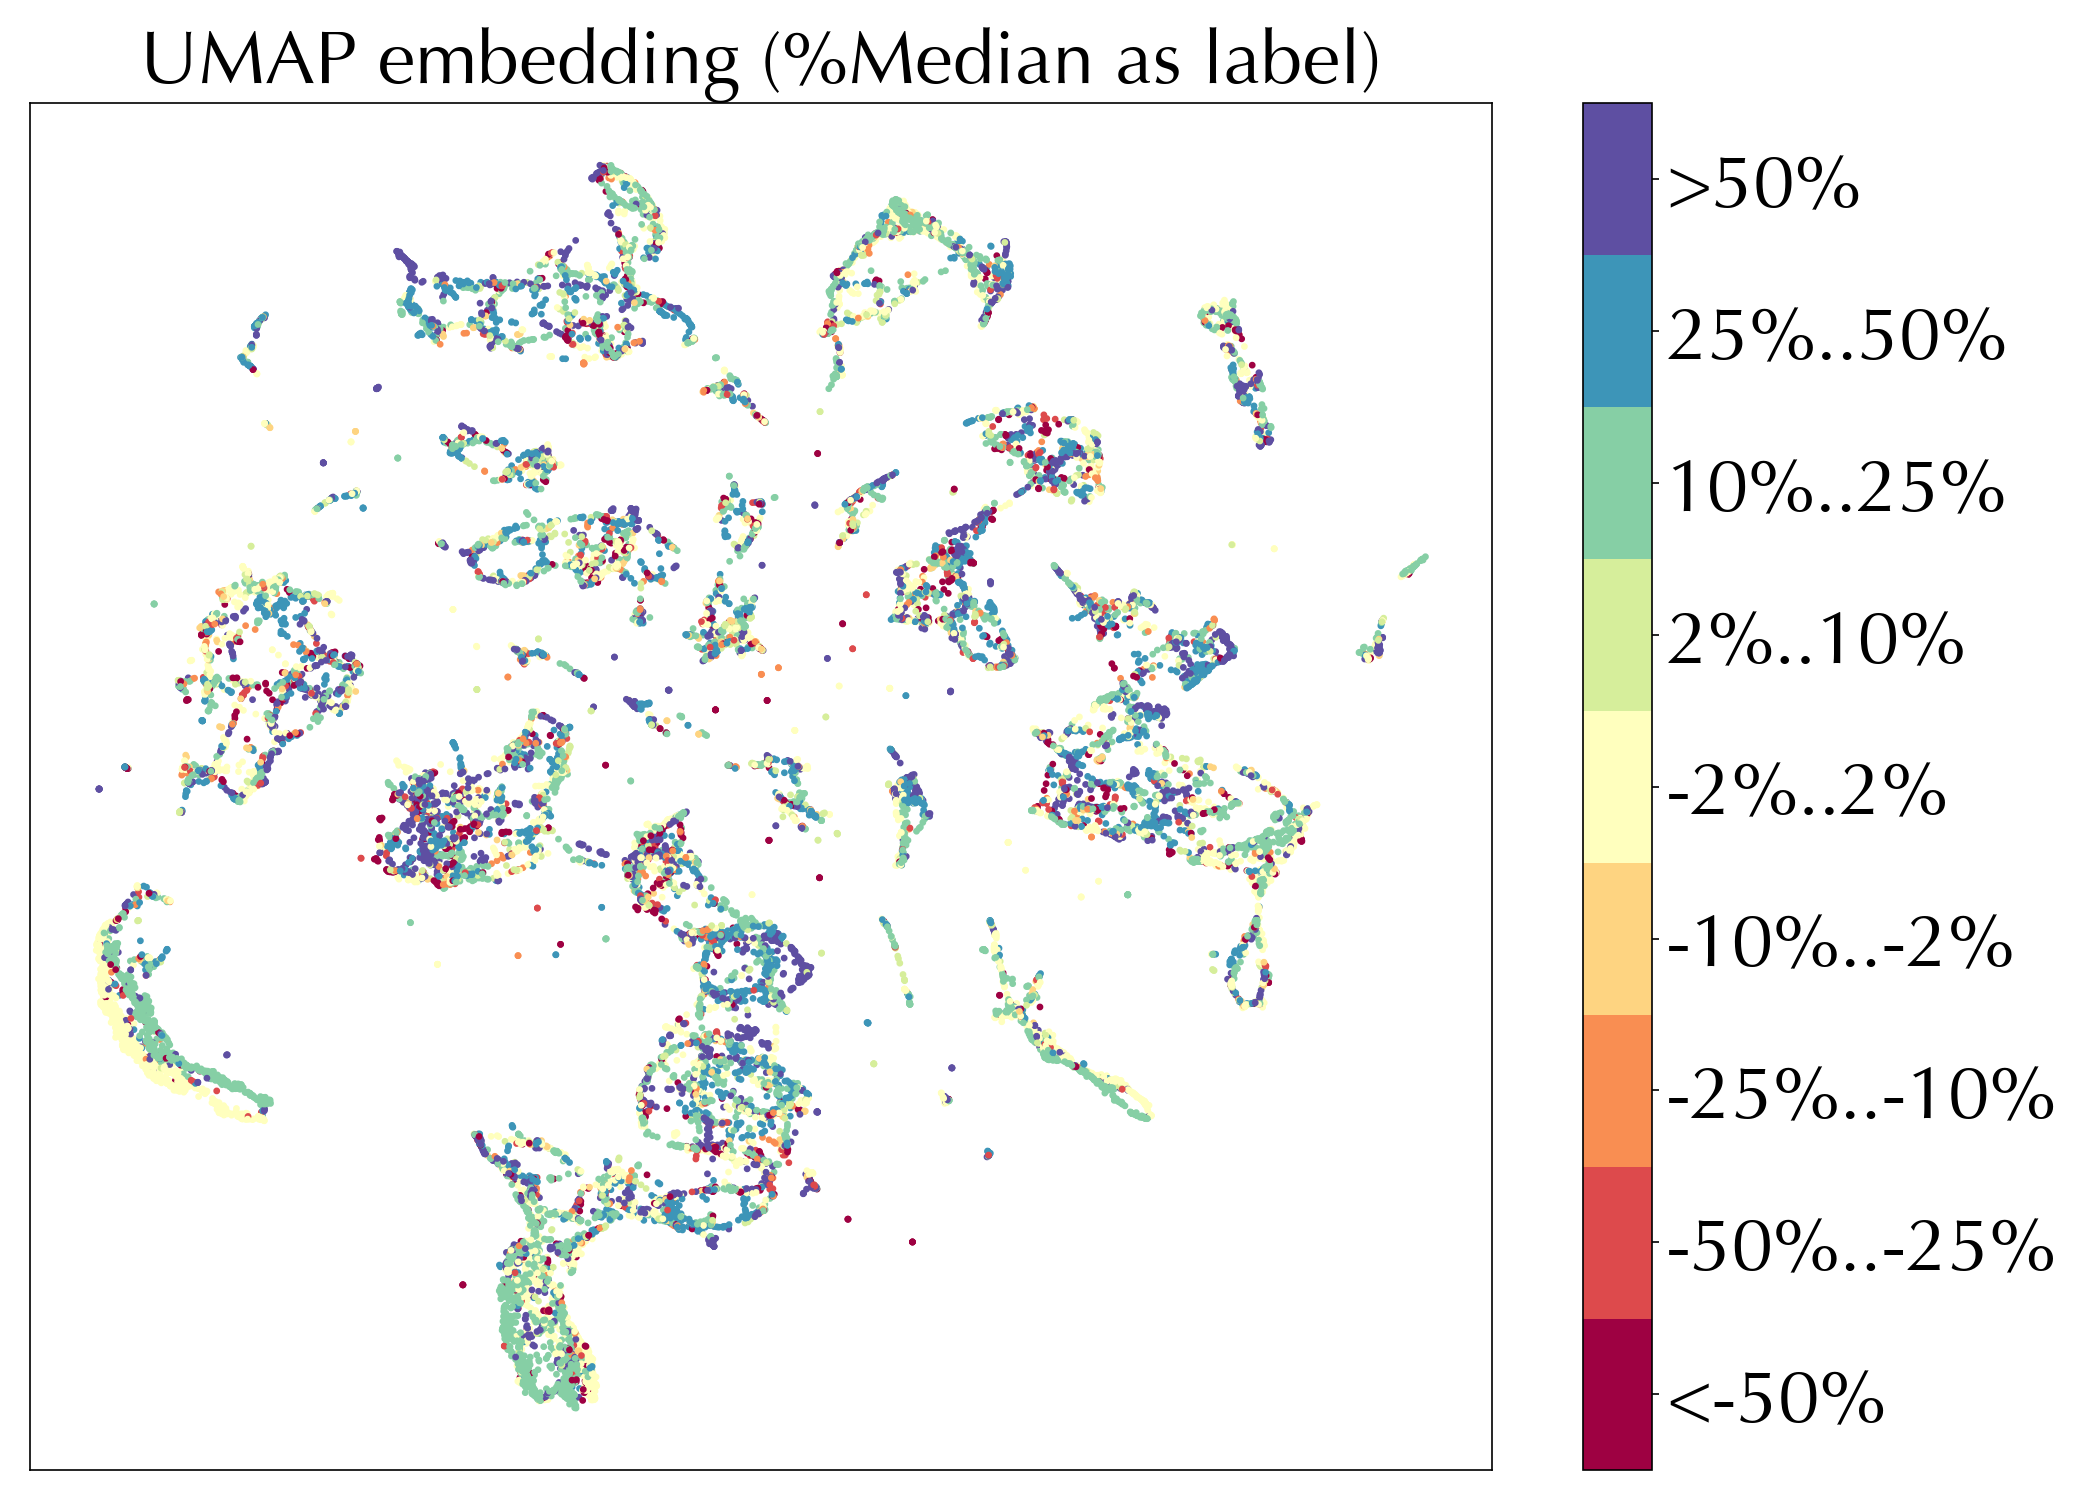
\includegraphics[width=0.99\linewidth]{images/umap-median.png}
    \captionof{figure}{UMAP dimension reduction of the data 
    using the median pay gap as a supervised label for manifold
    learning
    shows no clean separability in categories of data by pay gap severity.}
    \label{fig:manifold}
\end{centering}

To estimate whether models have a reasonable chance of fitting the data well, we performed a supervised manifold learning-based dimension reduction using UMAP \cite{mcinnes2018umap}. In this case, we have quantised the continuous regression target (the pay gap percentage) to form categorical labels such as \code{2\%..10\%}. The result, shown in Figure\ \ref{fig:manifold}, shows that the classes of pay gap severity are not easily separable, and finding an accurate continuous regressor may be difficult. 


\subsection{Models considered}
For the regression, our pipeline evaluates the following models:
\begin{description}
\item[Linear Regression] Used as baseline modelling indicator. It finds the line with the least squared difference to the target values. The result is a list of coefficients which determine the slope of the line, one for every feature of a training point together with an intercept which represents the bias of the line \cite{Pedregosa2011}.

\item[Random Forest] A supervised machine learning model that uses bagging technique. Bagging is an ensemble learning technique that in case of random forest runs multiple decision tress in parallel on sub-samples of the dataset and averages over them to give final predictions. This helps to overcome the problem of over-fitting or high variance in decision tree models \cite{Breiman2001a}. 

\item[Adaboost] A boosting ensemble model that fits weak learners on repeatedly modified data to produce the final prediction through weighted sum. Each training sample is assigned a weight on which the weak learners are trained to produce new re-weighted data \cite{adaboost}. 

\item[Gradient boosting] Another boosting algorithm that works sequentially with weak learners (decision tree models). In every iteration, it tries to minimise the loss function (e.g. least square, least absolute deviation) by adding a tree to finally add up to build a strong regression model \cite{Pedregosa2011}.

\item[Support vector regression] SVR is an application of SVM (support vector machine) to regression problem. Its purpose is to find a regression plane, so that all the data of a set is closest to that plane. The generalisation of SVM to SVR is realised by introducing a constant insensitive region called a square around the function. In this test tube, the optimisation problem is reconstructed to find the test tube which can best approximate the continuous value function, and the complexity of the model and the prediction error are balanced \cite{efficientLearningMachines}.

\item[Extreme Gradient Boosting (XGBoost)] XGBoost is a decision-tree-based ensemble model and an optimisation of the Gradient Boosting algorithm, which allows the use of Newton's method when optimising the loss function (with much faster convergence than gradient descent.) XGBoost also added a regularisation term in its loss function to control the complexity of the model. Column subsampling is supported in XGBoost which can reduce the chance of overfitting. Parallelisation in XGBoost makes training faster \cite{chen2016xgboost} .

\item[AutoML tools]
\label{sec:automl}
We also used an AutoML tool called TPOT. TPOT uses genetic programming to evolve a set of model candidates (from common models in the \code{scikit-learn} and \code{xgboost} libraries), along with their hyperparameters and combinations of feature pre-processing options (e.g. scaling) \cite{tpot-automl}. 

We used 10 generations with a population size of 150 models, which ran for more than five hours on a 4-core CPU. Our configuration for TPOT is shown in Appendix\ \ref{tpot-config}. As shown in Table\ \ref{tab:model-comparison-table}, TPOT did find models which were very slightly (0.1\%) more accurate than our best hand-tuned models. But they were considerably more complex, being pipelines of stacked models, and did not work with the model explainability tools we use in the next section, so we did not investigate them further.
\end{description}

\paragraph{Example of hand-tuning: Random Forest}
Each of the models has many tweakable hyperparameters which can be explored to improve default performance. Below we describe our experience with Random Forests as a representative example. 

The Random Forest model has many hyper-parameters of which we explored the following four:
\begin{description}
    \item[\code{max\_samples}], the number of samples used in each decision tree : the default of using the entire training set gave the best results and was kept same.
    \item[\code{n\_estimators}], the number of trees in the forest: Increasing the number of trees resulted in better accuracy up till 1500. 1000 was chosen as it improved the accuracy without taking too much training time.
    \item[\code{max\_features}], the number of features used in each split: After feature engineering, the data had 26 features in the input. The default is using all the features, however we got better accuracy with \code{sqrt}, i.e., 5 features for every split.
    \item[\code{max\_depth}], the depth of the tree: default was used that allows the tree to expand till the leaf nodes are pure or contain less samples than the \code{min\_samples\_split} if specified.
\end{description}

We could not improve the predictions for \code{DiffMeanHourlyPercent}, but hand-tuning the predictor for \code{DiffMeanHourlyPercent} score resulted in a modest (1.3\%) improvement.


\subsection{Model evaluation and selection}

Averaged scores for the 3-fold validation of the models is shown in Table\ \ref{tab:model-comparison-table}.

According to Occam’s Razor, the simplest model is the best, given similar predictive and explanatory power. To select one out of the many choices available for regression, we used coefficient of determination $R^2$, mean absolute error (MAE) and root mean squared error (RMSE) along with a visualisation of the correlation between predicted values and actual values. Explainable models were given priority (resulting in the elimination of the TPOT suggestions). 
% Random forest model scored the best at 0.77 for predicting median hourly pay gap and gradient boosting came second at $R^2$ 0.63 as shown in table \ref{tab:model-comparison-table}. 
We selected our best hand-tuned model (XGBoost) for further investigation.

\begin{centering}
    \scriptsize{
        \captionof{table}{A comparison of model performance. *AutoML models were complex pipelines of stacked regressors, which were not explored further because of the time
    cost of model search, for only a modest gain in performance. CV is the $R^2$ score run on the 
    cross-validation holdout set (10\% of companies that models
    never saw during training.) CV is only run for the best models.}
    \label{tab:model-comparison-table}
    \begin{tabular*}{\linewidth}{l|l|r|r|r|r} \hline
        Target & Model & MAE & RMSE & $R^2$ & CV \\ \hline
        \multirow{3}{4em}{Mean Pay Gap}
& Adaboost & 9.33 & 13.16 & 0.21 & - \\
& Decision Tree & 6.57 & 12.49 & 0.28& -  \\
& AutoML* & 5.30 & 9.32 & 0.63& -  \\
& Gradient Boosting & 5.79 & 9.80 & 0.57& -  \\
& Linear Regression & 6.31 & 10.41 & 0.51& -  \\
& Random forest & 5.55 & 9.48 & 0.60& -  \\
& SVR & 6.00 & 10.27 & 0.53& -  \\
& {\bf XGBoost} & 5.25 & 9.22 & {\bf 0.62} & 0.45  \\ \hline
        \multirow{3}{4em}{Median Pay Gap}
& Adaboost & 8.71 & 12.16 & 0.40 & -  \\
& Decision Tree & 6.93 & 11.32 & 0.48  & -\\
& AutoML* & 5.55 & 8.94 & 0.68 & - \\
& Gradient Boosting & 6.06 & 9.55 & 0.63  & -\\
& Linear Regression & 6.55 & 9.93 & 0.60 & - \\
& Random forest & 5.72 & 9.19 & 0.66 & - \\
& SVR & 6.31 & 10.16 & 0.58 & - \\
& {\bf XGBoost} & 5.41 & 8.87 & {\bf 0.68} & 0.62\\ \hline
    \end{tabular*}}
\end{centering}



\subsection{Model interpretation and explainabality}
Predicting the pay gap from these descriptive statistics and company features is
not directly useful -- it is difficult to think of a situation in which one would have the input data but not the GPG information itself. But building explainable predictive models allows us to gain an insight into which features are affecting GPG and how. We note that this does not equate to rigorous causal modelling.

\begin{centering}
    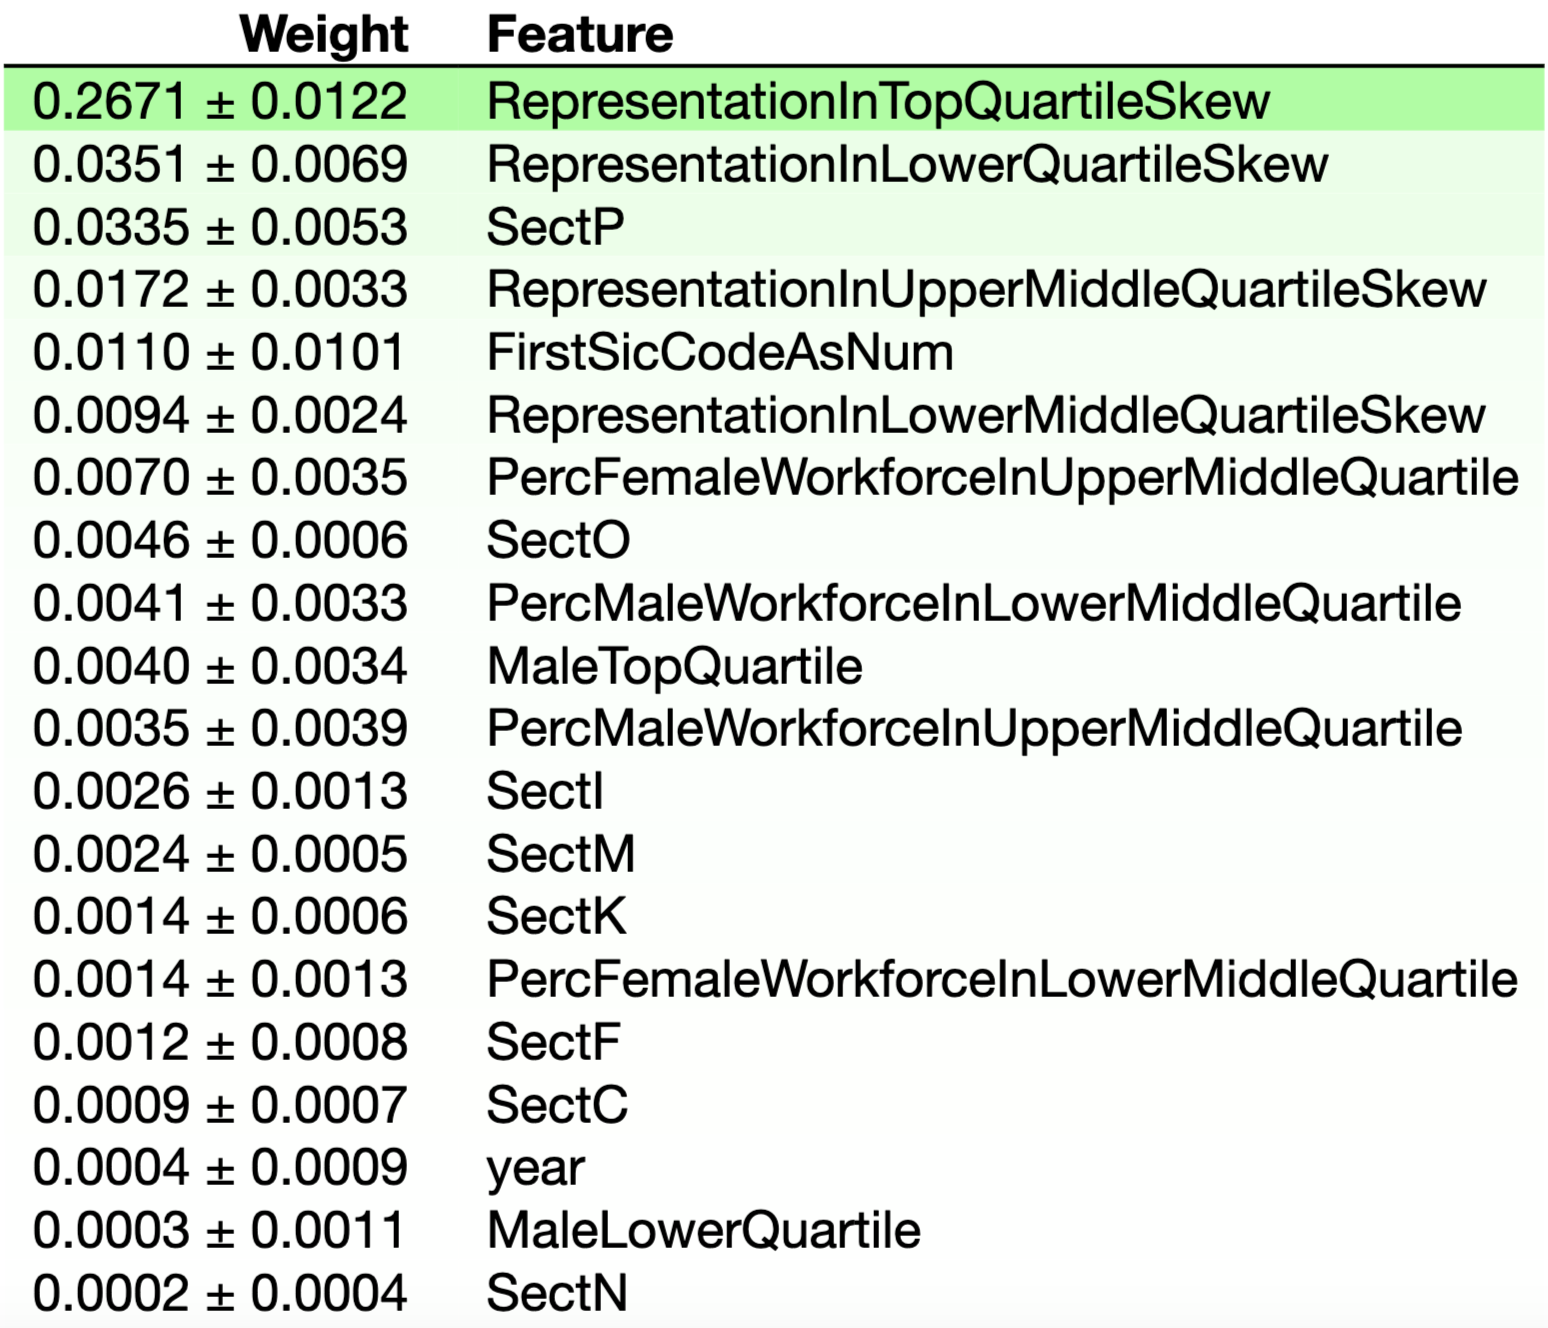
\includegraphics[width=0.99\linewidth]{images/PI-with-extra-features.png}
    \captionof{figure}{Feature weights for predicting median pay gap calculated through permutation importance for XGBoost model}
    \label{fig:median-rf-pi}
\end{centering}

In order to find out which features affected the predictions most and in which direction, we used permutation importance, partial dependence plots and SHAP values \cite{Molnar2020}.
Permutation importance is calculated by getting predictions from the fitted model on the validation sets by shuffling one feature column at a time \cite{Altmann2010}. If a feature that had a lot of influence on the model is made redundant through shuffling, there will be significant performance loss. 
The weights in Figure \ref{fig:median-rf-pi} denote the decrease in accuracy of the model on shuffling corresponding feature, repeated multiple times to account for randomness.
Using permutation importance, it was discovered that the representation skew in the lower and top quartiles formed the biggest predictors as shown in Figure \ref{fig:median-rf-pi}. 
It is worth noting that the employer size is one of the least important features here due to the imbalance in the data in each category of \code{EmployerSize} as can be seen in Figure \ref{fig:employer-size-dist}.


With partial dependence plots, we plot the variation in the most important features found through permutation importance, the \code{RepresentationInLowerQuartileSkew} and \code{RepresentationInTopQuartileSkew} and their effect on the prediction, here median pay gap as depicted in Figure \ref{fig:pdp-median-rf} and \ref{fig:pdp-top-median-rf}. Through the PDP plots we can see a linear relation between GPG and the skew of representation of women in the top and lower pay quartiles.

\begin{centering}
    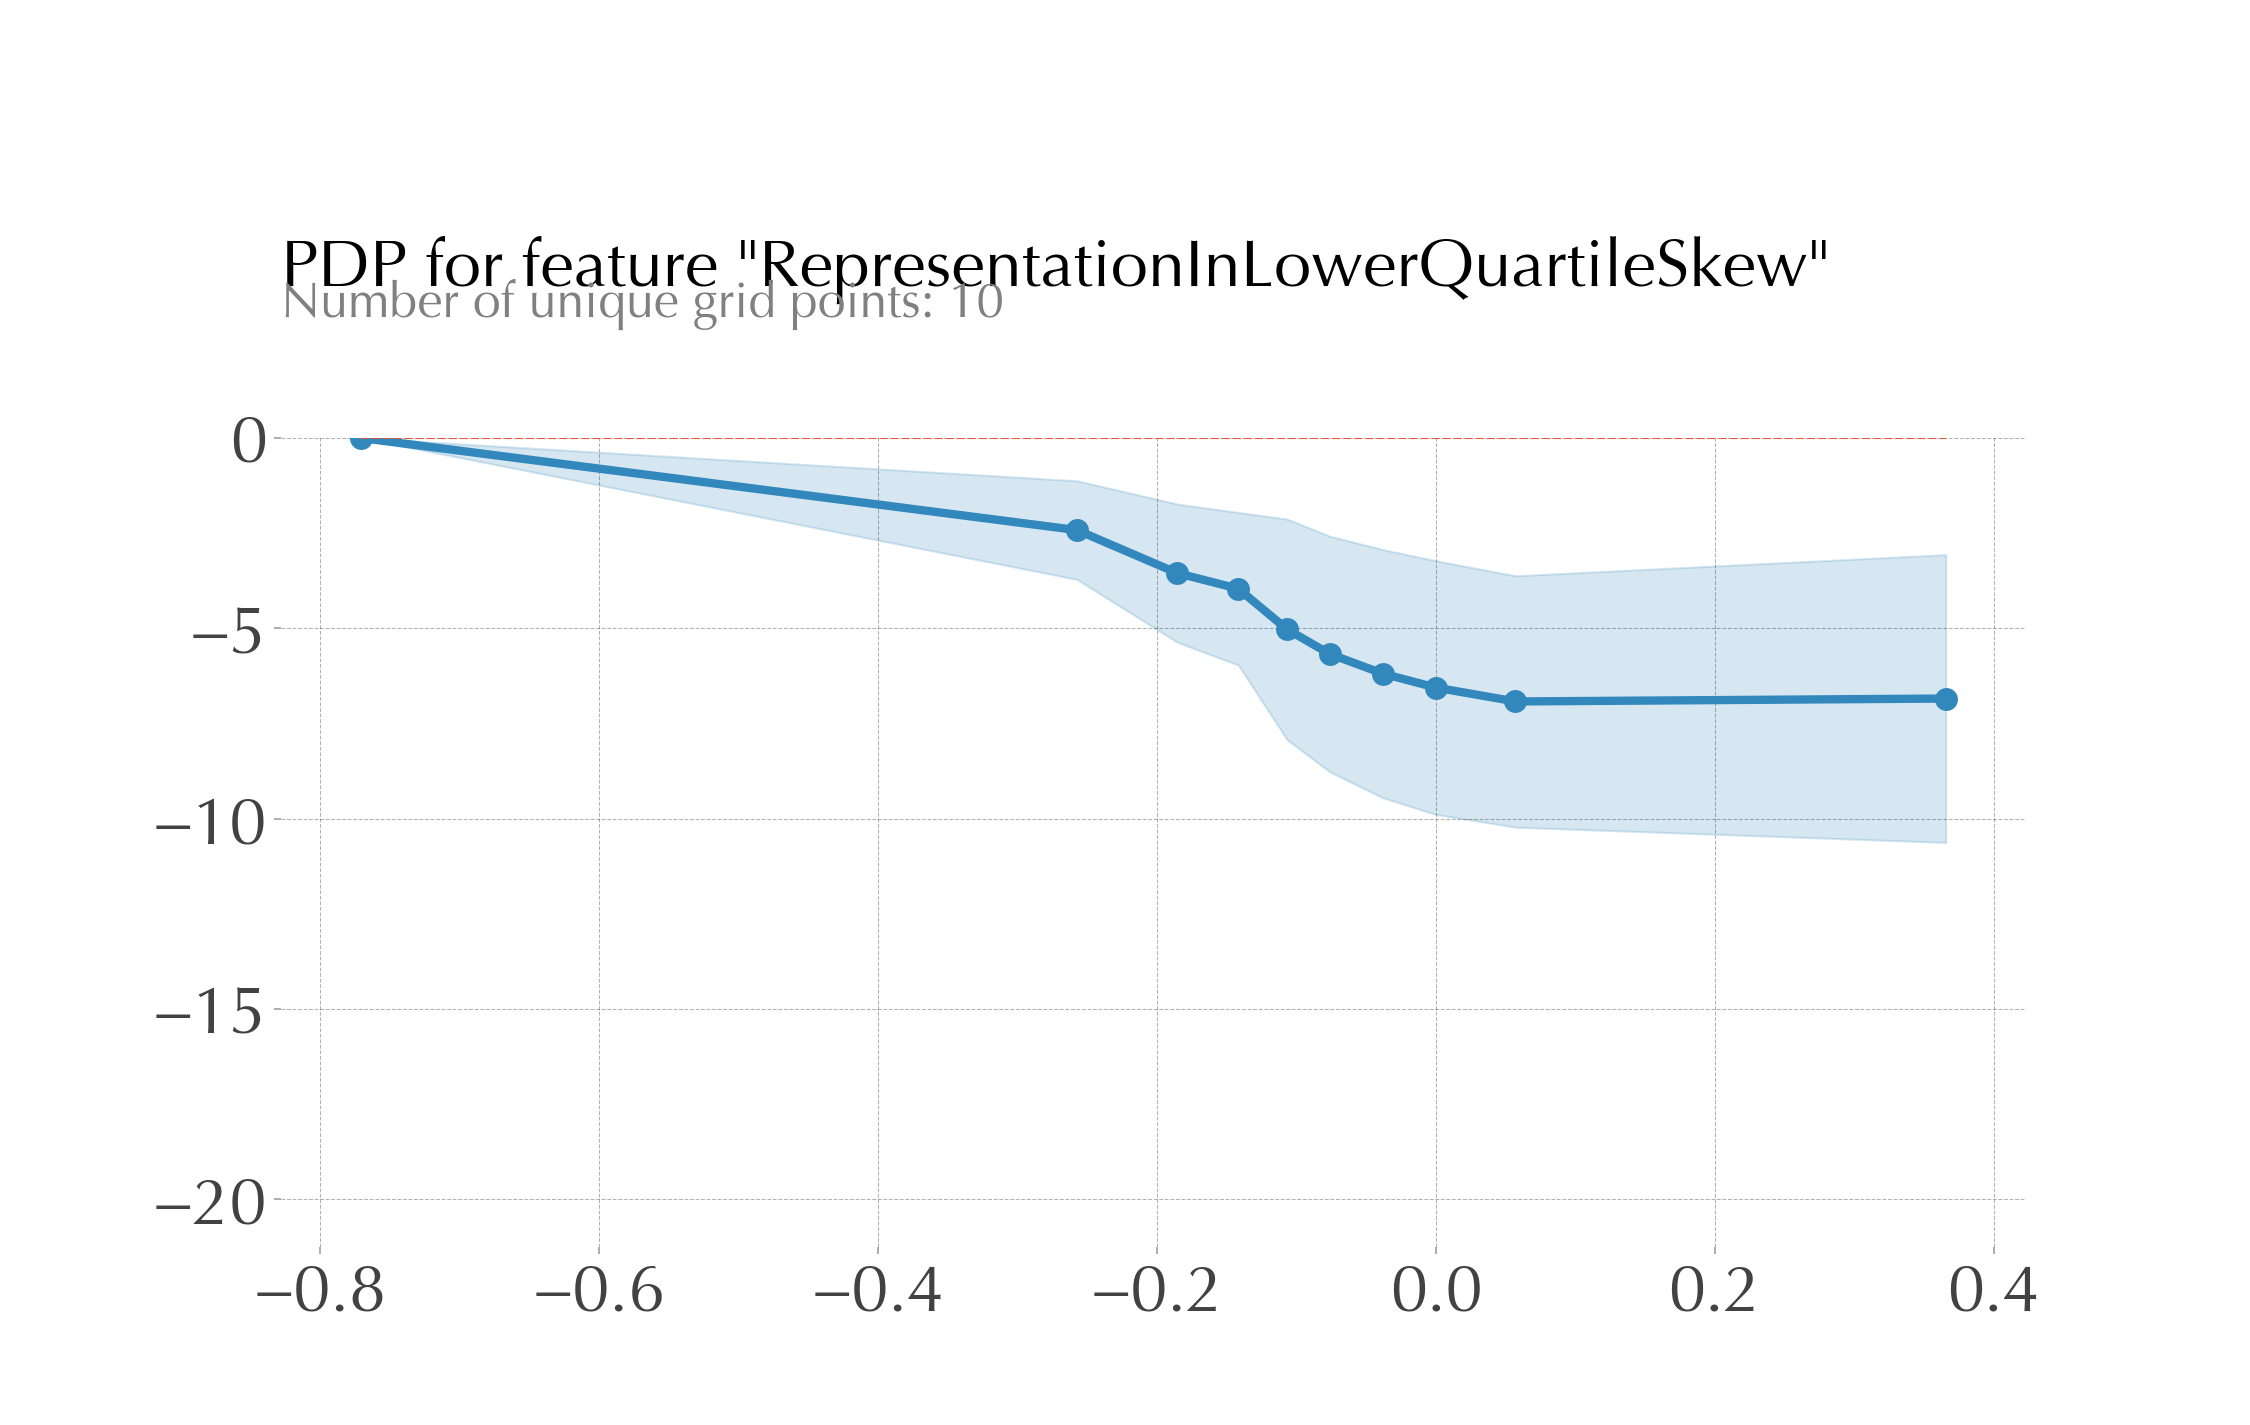
\includegraphics[width=1.1\linewidth]{images/DiffMedianHourlyPercent-RepresentationInLowerQuartileSkew-pdp.png}
    \captionof{figure}{\code{RepresentationInLowerQuartileSkew} feature's effect on XGBoost model for median GPG prediction. Equal representation of men and women in lower quartile corresponds to lower GPG.}
    \label{fig:pdp-median-rf}
\end{centering}

\begin{centering}
    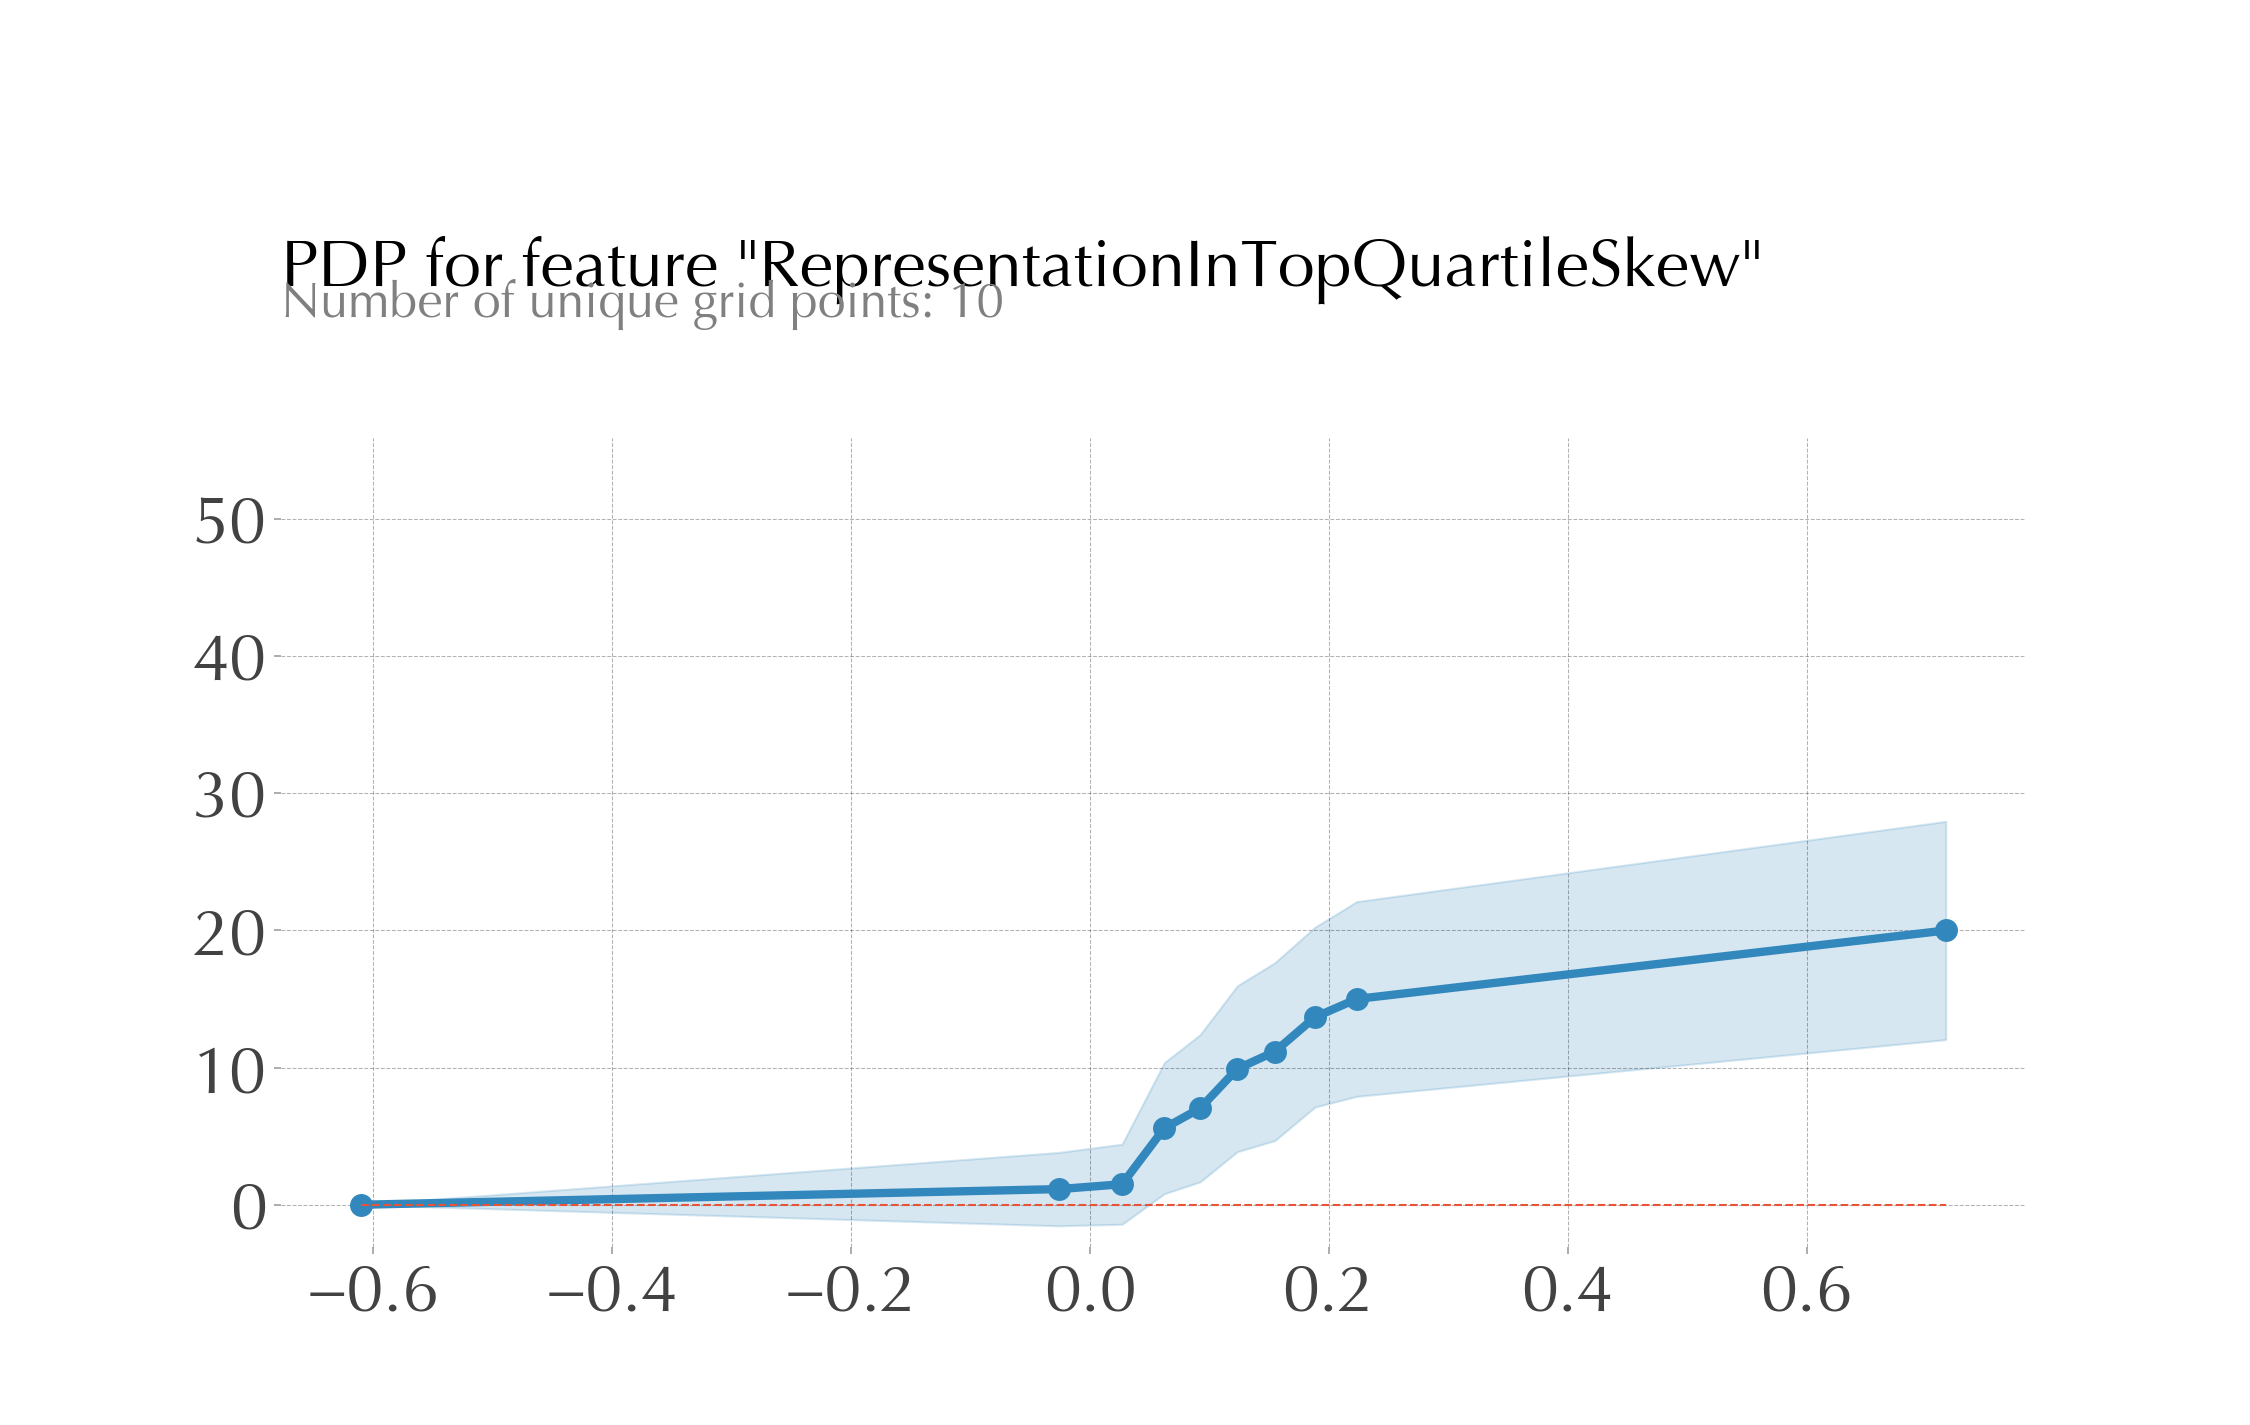
\includegraphics[width=1.1\linewidth]{images/DiffMedianHourlyPercent-RepresentationInTopQuartileSkew-pdp.png}
    \captionof{figure}{\code{RepresentationInTopQuartileSkew} feature's effect on XGBoost model for median GPG prediction. More representation of men in the top quartile leads to an increase in the GPG.}
    \label{fig:pdp-top-median-rf}
\end{centering}

SHAP values, Shapley Additive explanations \cite{Lundberg2017}, can be used to find the effect of each feature on single predictions. It is calculated using a baseline value for prediction compared to the actual prediction and returns how much each feature contributed to the difference.

\begin{figure*}
    \centering
    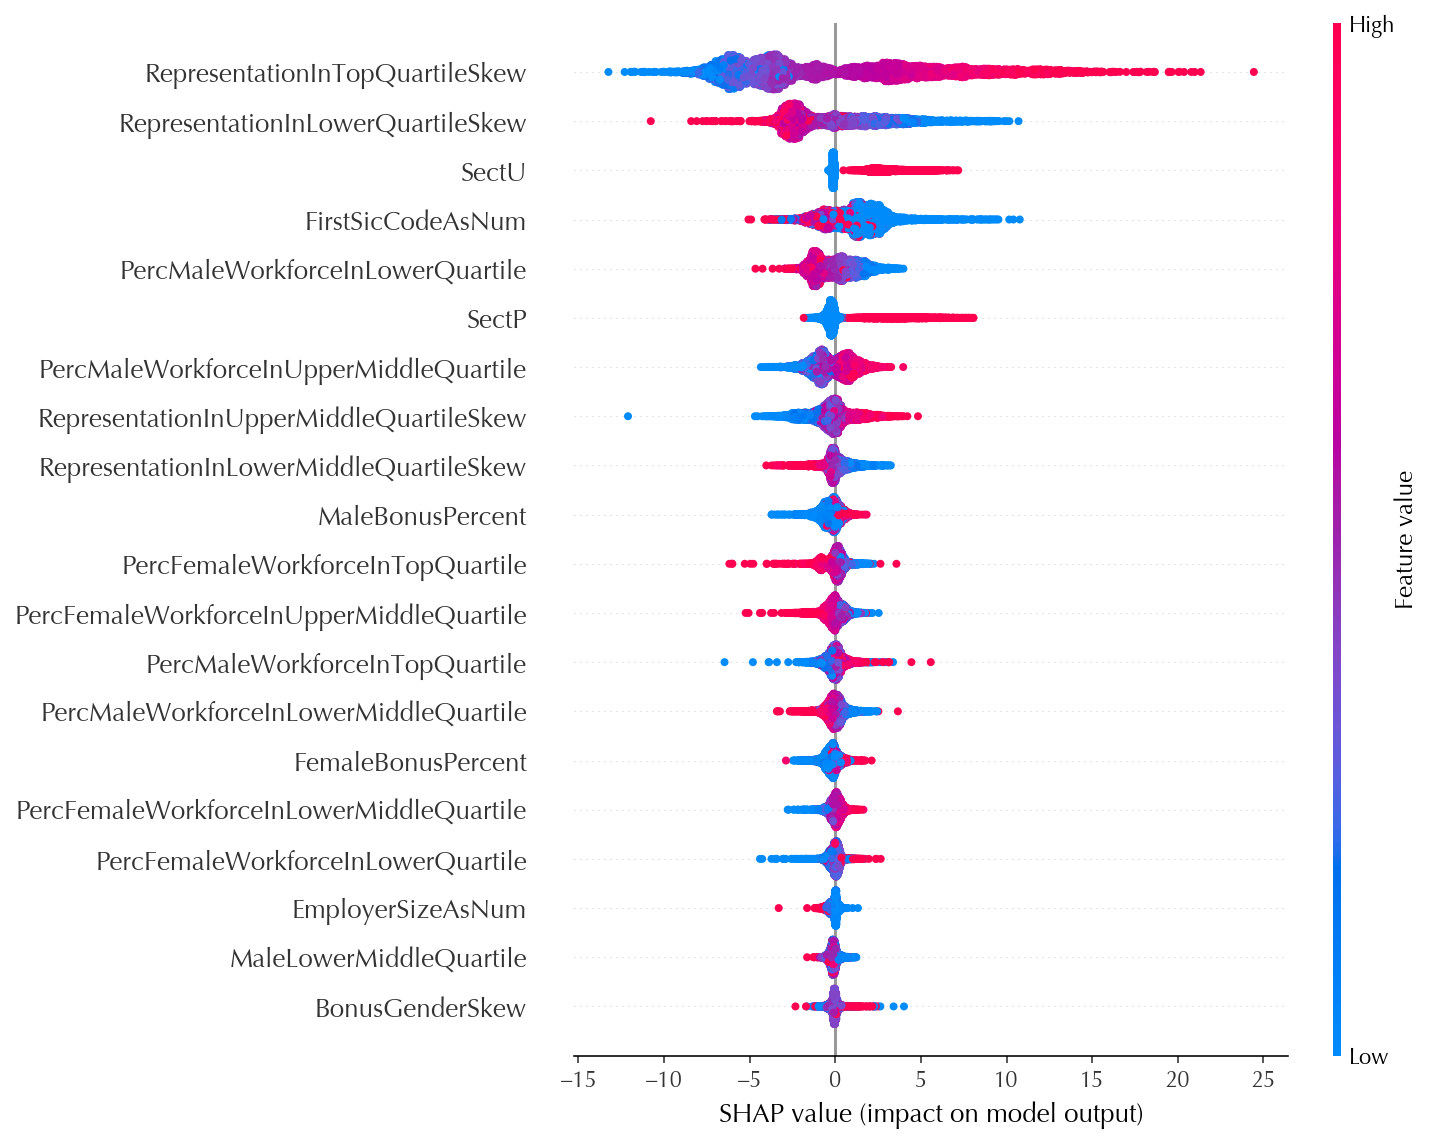
\includegraphics[width=0.7\textwidth]{images/median-shap.png}
    \captionof{figure}{Summary plot of SHAP values for XGBoost model for median GPG prediction on validation data.}
    \label{fig:shap-median-rf}
\end{figure*}

A summary plot of SHAP values in Figure \ref{fig:shap-median-rf} shows that the a skew of the representation of employees in the top quartile towards men results in an increase in the predicted pay gap. An increased representation of female employees in the top quartile reduces the pay gap estimate. We can also see that some sectors like SectU (Activities of extraterritorial organisations and bodies) and SectP (Education) are prominent in the plot, indicating that these sectors almost always have a pay gap albeit small. Since the holdout dataset is comparatively smaller than the full dataset, we acknowledge that not all sectors may be completely represented by it.


\subsection{Analysis of predictions}
Our best model can detect outliers based on the difference in representation of employees by gender. We used the holdout dataset to dig deeper the model's mispredictions. 30\% of the companies in the holdout set had not provided an internal report link for their GPG and of the 70\% that had, some of the links to the reports redirected to the company website or were dead links. Nevertheless, we obtained some detailed reports from companies that appeared to be outliers according to our median pay gap model. In \cite{PenkValleyAcademyTrust2019}, \cite{Aquinastrust2019} and \cite{ElevateMultiAcademyTrust2020}, we found a huge median GPG was reported (45 - 64\%) despite an overwhelming number of women in each quartile. These trusts' reports attributed the GPG to more women working in support staff roles, which are paid less than full-time roles. Hence, we posit that more indicators like full-time vs part-time metrics are required to better model the data for GPG prediction. What is not clear by these reports is that how is this difference not balanced by more women to men ratio in their top quartile. The ratio of women to men in each quartile is an insufficient predictor, and our derived features, like representation skew for women, can better explain the GPG in such cases by showing the percentage of women at each level compared to all women in the company.


